\problem{What is a constant delay filter? Where is it important? What are the techniques of getting a
filter with almost constant delay? Explain.}
A constant delay filter is a filter that gives output delayed in time from input signal. The input and output signal differs by constant time hence the name constant delay filter.
\begin{figure}[H]
    \centering
    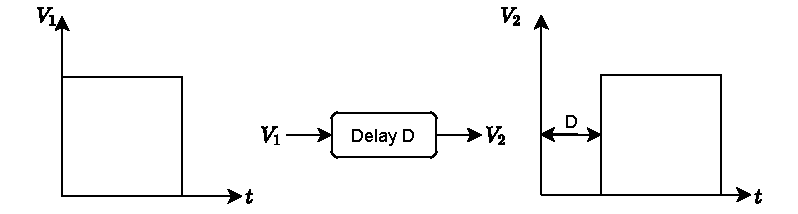
\includegraphics{../Figures/delay.pdf}
    \caption{Constant delay filter}
    \label{fig:const-delay}
\end{figure}
The relation between output and input  is thus given as,
\begin{equation*}
        V_2(t)-V_1(t-D)
\end{equation*}
If $V_1(t)=A\sin(\omega t + \Phi)$ then  $V_2(t)=A\sin(\omega t -\omega D + \Phi)$. So, the two signal differ by phase angle of $\theta=-\omega D$, i.e. $\ddfrac{V_2}{V_1}=1\angle -\omega D$. Hence the transfer function is given as,
\begin{equation*}
    |T|=\frac{V_2}{V_1}=e^{-j\omega D}=e^{-sD}
\end{equation*}
For normalized delay $D=1$, 
\begin{equation}
    |T|=e^{-s}
    \label{eqn:delay-tfr}
\end{equation}
\begin{figure}[H]
    \centering
    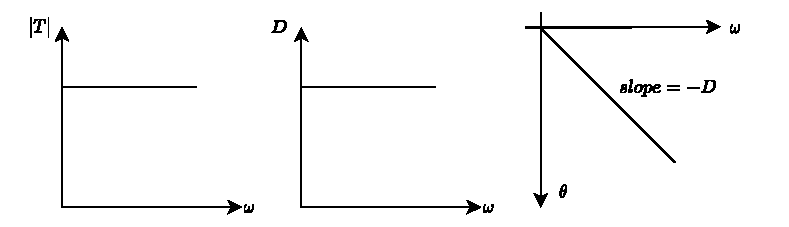
\includegraphics{../Figures/delay_plot.pdf}
    \caption{Requirement for constant delay and no distortion}
    \label{fig:const-delay-plot}
\end{figure}
For linear phase with negative slope and constant magnitude, the delay will be constant. Similarly, the obtained signal will be distortionless. Such filter is important in signal processing application for mostly analog video signals and other applications where a constant group delay is prioritized rather than the response.\\
Since the transfer function given in Equation~\ref{eqn:delay-tfr} can't be realized with lumped elements, the design is approximated in quotient of polynomials. The techniques used to approximate the constant delay filters are explained in brief.
\subsubsection*{Bessel-Thomson}
In this method, an all pole transfer function is assumed, using which the corresponding delay is calculated. Then the series is expanded using Taylor series and vanishing conditions for the coefficients are determined to complete the approximation.\\
If we assume an all pole second order transfer function as,
\begin{equation*}
    \begin{aligned}
        &T_2(s)=\frac{a_0}{s^2+a_1s+a_0}\\
        &\Rightarrow T_2(j\omega)=\frac{a_0}{-\omega^2+ja_1\omega+a_0}\\
        &\therefore \theta=-\tan^{-1}\left(\frac{a_1\omega}{a_0-\omega^2}\right)\\
        &\because D=\frac{-d\theta}{d\omega}=\frac{d}{d\omega}\left[tan^{-1}\left(\frac{a_1\omega}{a_0-\omega^2}\right)\right]\\
        &\Rightarrow D=\ddfrac{d\left[tan^{-1}\left(\frac{a_1\omega}{a_0-\omega^2}\right)\right]}{d\left[\frac{a_1\omega}{a_0-\omega^2}\right]}\times\ddfrac{d\left[\frac{a_1\omega}{a_0-\omega^2}\right]}{d\omega}\\
        &\Rightarrow D=\ddfrac{1}{1+\left(\frac{a_1\omega}{a_0-\omega^2}\right)^2}\times\ddfrac{\left(a_0-\omega^2\right)\frac{d(a_1\omega)}{d\omega}-a_1\omega\frac{d(a_0-\omega^2)}{d\omega}}{(a_0-\omega^2)^2}\\
        &\Rightarrow D=\frac{(a_0-\omega^2)^2}{(a_0-\omega^2)^2+(a_1\omega)^2}\times\frac{a_1(a_0-\omega^2)-a_1\omega(-2\omega)}{(a_0-\omega^2)^2}\\
        &\Rightarrow D=\frac{a_1(a_0-\omega^2)+2a_1\omega^2}{(a_0-\omega^2)^2+(a_1\omega)^2}\\
        &\Rightarrow D=\frac{a_1(a_0+\omega^2)}{a_0^2+(a_1^2-2a_0)\omega^2+\omega^4}\\
        &\Rightarrow D=\left(\frac{a_1}{a_0}\right)\times\ddfrac{1+\frac{\omega^2}{a_0}}{1+\left(\frac{a_1^2}{a_0^2}-\frac{2}{a_0}\right)\omega^2+\frac{\omega^4}{a_0^2}}
    \end{aligned}
\end{equation*}
Using taylor series to expand as,
\begin{equation*}
    D=\left(\frac{a_1}{a_0}\right)\left[1+\left(\frac{1}{a_0}-\frac{a_1^2}{a_0^2}+\frac{2}{a_0}\right)\omega^2+\cdots\right]
\end{equation*}
The condition for the second term to vanish is,
\begin{equation*}
   \begin{aligned}
    &\Rightarrow \frac{3}{a_0}=\frac{a_1^2}{a_0^2}\\
    &\Rightarrow 3a_0=a_1^2\\
    &\Rightarrow a_0=a_1=3 \quad [\text{To normalize D, set }a_0=a_1] 
   \end{aligned}
\end{equation*}
Using these values, we get,
\begin{equation*}
    T_2(s)=\frac{3}{s^2+3s+3}
\end{equation*}
The corresponding delay is given as,
\begin{equation*}
    D_2(\omega)=\ddfrac{\left(1+\frac{\omega^2}{3}\right)}{\left(1+\frac{\omega^2}{3}+\frac{\omega^4}{9}\right)}=\frac{3\omega^2+9}{\omega^4+3\omega^2+9}
\end{equation*}
\subsubsection*{Storch Method}
In this method, the transfer function in equation~\ref{eqn:delay-tfr} is approximated using hyperbolic expansion as,
\begin{equation*}
    \begin{aligned}
        &T(s)=e^{-s}=\frac{1}{e^s}\\
        &\Rightarrow T(s)=\frac{1}{\sinh s +\cosh s}\\
        &\Rightarrow T(s)=\ddfrac{\frac{1}{\sinh s}}{\frac{\sinh s + \cosh s}{\sinh s}}\\
    \end{aligned}
\end{equation*}
The hyperbolic expansion is given as,
\begin{equation*}
    \begin{aligned}
        &\cosh s =1+\frac{s^2}{2!}+\frac{s^4}{4!}+\frac{s^6}{6!}+\cdots\\
        &\sinh s =1+\frac{s^3}{3!}+\frac{s^5}{5!}+\frac{s^7}{7!}+\cdots\\
    \end{aligned}
\end{equation*}
To obtain $\coth s$, we divide $\cosh s$ by $\sinh s$ then inverting and repeating the division as,
\begin{equation*}
    \coth s =\frac{1}{s}+\ddfrac{1}{\frac{3}{s}+\ddfrac{1}{\frac{5}{s}+\ddfrac{1}{\frac{7}{s}+\cdots}}}
\end{equation*}
For $n$ take $n$ steps, i.e. for $n=2$, we take two steps as,
\begin{equation*}
    \coth s =\frac{1}{s}+\ddfrac{1}{\frac{3}{s}}=\frac{1}{s}+\frac{s}{3}=\frac{s^2+3}{3s}
\end{equation*}
Adding numerator and denominator, we get,
\begin{equation*}
    D_2(s)=s^2+3s+3
\end{equation*}
The transfer function is then given as,
\begin{equation*}
    T_2(s)=\frac{D_2(0)}{D_2(s)}=\frac{3}{s^2+3s+3}
\end{equation*}